% Large-field DFS with Upside CVaR: 15-minute progress presentation.
%
% Build from this folder:   latexmk -pdf slides.tex
% Figures come from results/figures/ (python run_all.py, then python make_figures.py,
% from the repository root).
%
% Timing guide (about 15 minutes, plus questions):
%   1. The problem ............. slides 3-5   ~3 min
%   2. Our approach ............ slides 6-9   ~4.5 min
%   3. Early results ........... slides 10-13 ~5 min
%   4. What is next ............ slides 14-16 ~2.5 min

% Shared styling for slides.tex and backup.tex.

\documentclass[aspectratio=169,11pt]{beamer}

\usepackage[T1]{fontenc}
\usepackage{lmodern}
\usepackage{amsmath,amssymb}
\usepackage{booktabs}
\usepackage{tikz}
\usetikzlibrary{arrows.meta,positioning,fit}

\graphicspath{{figures/}{../results/figures/}}

% ------------------------------------------------------------------ appearance
\definecolor{navy}{RGB}{23,50,94}
\definecolor{accent}{RGB}{31,119,180}
\definecolor{good}{RGB}{44,160,44}
\definecolor{warn}{RGB}{214,39,40}
\definecolor{soft}{RGB}{240,244,250}
\setbeamercolor{frametitle}{fg=navy}
\setbeamercolor{title}{fg=navy}
\setbeamercolor{structure}{fg=accent}
\setbeamercolor{block title}{bg=navy,fg=white}
\setbeamercolor{block body}{bg=soft}
\setbeamerfont{frametitle}{series=\bfseries,size=\large}
\setbeamertemplate{navigation symbols}{}
\setbeamertemplate{itemize items}[circle]
\setbeamertemplate{blocks}[rounded][shadow=false]
\setbeamertemplate{footline}{%
  \hfill\usebeamercolor[fg]{structure}\scriptsize\insertframenumber\,/\,\inserttotalframenumber\hspace{1em}\vspace{0.6em}}
\AtBeginSection[]{%
  \begin{frame}[plain,noframenumbering]
    \centering\vfill
    {\Large\bfseries\color{navy}\insertsectionnumber.\ \insertsection}\par\vfill
  \end{frame}}

\newcommand{\E}{\mathbb{E}}
\newcommand{\hl}[1]{\textcolor{accent}{\textbf{#1}}}
\newcommand{\ucvar}{\operatorname{U\text{-}CVaR}}
\newcommand{\bigstat}[2]{%
  \begin{minipage}[t]{\linewidth}\centering
    {\LARGE\bfseries\color{navy}#1}\par\vspace{0.3em}
    {\footnotesize #2\par}
  \end{minipage}}


\title{Playing for the Top 0.1\,\%}
\subtitle{Simulating large-field Daily Fantasy Sports contests\\
  and building lineups with Upside CVaR}
\author{Benjamin Minkin \and Marcus Minutello \and Alex Dolce}
\institute{AMS 553 / CSE 529: Simulation and Modeling \quad (work in progress)}
\date{}

\begin{document}

% ======================================================================
\begin{frame}[plain]
  \titlepage
\end{frame}

\begin{frame}{Roadmap}
  \begin{enumerate}
    \setlength\itemsep{0.8em}
    \item \textbf{The problem:} why winning a top-heavy contest is not about expected points
    \item \textbf{Our approach:} a three-stage simulation and an Upside-CVaR objective
    \item \textbf{Early results:} validation, a strategy comparison, over-fitting, and
      importance sampling
    \item \textbf{What is next:} limitations and our plan to the final report
  \end{enumerate}
\end{frame}

% ======================================================================
\section{The problem}

% ~1 min
\begin{frame}{Large-field DFS: draft 9 players, beat thousands of strangers}
  Contests like DraftKings' NFL Millionaire Maker draw hundreds of thousands of entries.
  Each entry picks a QB, 2 RB, 3 WR, a TE, a FLEX (RB/WR/TE) and a defense under a
  \$50{,}000 salary cap, and scores the real players' fantasy points.
  \vspace{1.6em}

  \begin{columns}[t]
    \begin{column}{0.24\textwidth}
      \bigstat{10,001}{entries in our simulated contest (real ones: 100k--400k)}
    \end{column}
    \begin{column}{0.24\textwidth}
      \bigstat{26\,\%}{of the prize pool goes to the top 10 entries (top 0.1\,\%)}
    \end{column}
    \begin{column}{0.24\textwidth}
      \bigstat{20\,\%}{of entries cash at all; minimum cash \$2.15 on a \$1 entry}
    \end{column}
    \begin{column}{0.24\textwidth}
      \bigstat{$-15\,\%$}{average return: the house keeps a 15\,\% rake}
    \end{column}
  \end{columns}
  \vfill
  {\scriptsize\color{navy} Payouts: top 20\,\% paid; minimum cash plus a power-law bonus,
  calibrated so 1st place takes 10\,\% of the pool.\par}
\end{frame}

% ~1 min
\begin{frame}{Maximizing expected points $\neq$ maximizing expected payout}
  \begin{columns}[t]
    \begin{column}{0.32\textwidth}
      \begin{block}{You need a boom}
        The money is in the top 0.1\,\%. Even the best-projected lineup usually lands far
        below that line, so we want a high \emph{best case}, not just a high average.
      \end{block}
    \end{column}
    \begin{column}{0.32\textwidth}
      \begin{block}{Stacks add upside}
        A quarterback and his own receivers rise and fall together. That correlation adds
        variance, and variance produces winning weeks.
      \end{block}
    \end{column}
    \begin{column}{0.32\textwidth}
      \begin{block}{The field sets the bar}
        The winning score depends on what everyone else drafted. A popular player who
        booms lifts the whole field; an unpopular one lifts only you.
      \end{block}
    \end{column}
  \end{columns}
  \vspace{1.5em}
  \textbf{Our question:} can a lineup chosen for its \hl{upper tail} (Upside CVaR) beat
  lineups chosen for expected points, by a statistically significant margin?
\end{frame}

% ~1 min
\begin{frame}{Building on Haugh \& Singal (2019)}
  \begin{columns}[c]
    \begin{column}{0.56\textwidth}
      \begin{itemize}
        \setlength\itemsep{0.6em}
        \item Model the \hl{opponents}, not just the players
        \item Each position's ownership follows a \textbf{Dirichlet-multinomial} model,
          plus a probability $q$ that an opponent stacks QB and WR
        \item Opponent lineups drawn by \textbf{acceptance--rejection}: keep only legal
          lineups that spend most of the cap
        \item Lineups chosen by mean--variance optimization against the simulated
          winning score
      \end{itemize}
    \end{column}
    \begin{column}{0.4\textwidth}
      \bigstat{$\sim$4$\times$}{expected P\&L from modeling opponents in top-heavy contests
      (about \$1{,}400 $\to$ \$6{,}000 over the 2017 NFL season)}
      \vspace{1.2em}

      \bigstat{3$\times$}{realized profit of their strategic portfolio vs.\ the benchmark
      (\$280 over 17 weeks)}
    \end{column}
  \end{columns}
  \vfill
  {\scriptsize M.\,B. Haugh and R. Singal, \emph{How to Play Fantasy Sports Strategically
  (and Win)}, 2019.\par}
\end{frame}

% ======================================================================
\section{Our approach}

% ~1 min
\begin{frame}{Three simulation stages, then pick a lineup for its upside}
  \centering
  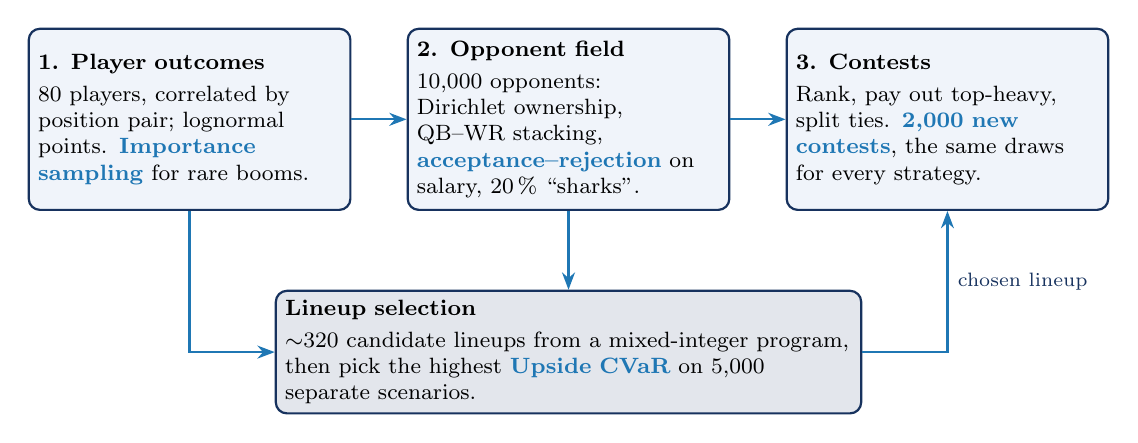
\begin{tikzpicture}[
      box/.style={draw=navy,thick,rounded corners,fill=soft,text width=3.85cm,
                  minimum height=2.3cm,align=left,font=\footnotesize,
                  execute at begin node={\hyphenpenalty=10000\exhyphenpenalty=10000}},
      sel/.style={draw=navy,thick,rounded corners,fill=navy!12,text width=7.2cm,
                  align=left,font=\footnotesize,
                  execute at begin node={\hyphenpenalty=10000\exhyphenpenalty=10000}},
      flow/.style={-{Stealth[length=2.2mm]},thick,accent}]
    \node[box] (s1) {\textbf{1. Player outcomes}\\[2pt]
      80 players, correlated by position pair; lognormal points.
      \hl{Importance sampling} for rare booms.};
    \node[box,right=0.7cm of s1] (s2) {\textbf{2. Opponent field}\\[2pt]
      10{,}000 opponents: Dirichlet ownership, QB--WR stacking,
      \hl{acceptance--rejection} on salary, 20\,\% ``sharks''.};
    \node[box,right=0.7cm of s2] (s3) {\textbf{3. Contests}\\[2pt]
      Rank, pay out top-heavy, split ties. \hl{2{,}000 new contests}, the same draws for
      every strategy.};
    \draw[flow] (s1) -- (s2);
    \draw[flow] (s2) -- (s3);
    \node[sel,below=1.0cm of s2] (opt) {\textbf{Lineup selection}\\[2pt]
      $\sim$320 candidate lineups from a mixed-integer program, then pick the highest
      \hl{Upside CVaR} on 5{,}000 separate scenarios.};
    \draw[flow] (s1.south) |- (opt.west);
    \draw[flow] (s2.south) -- (opt.north);
    \draw[flow] (opt.east) -| node[pos=0.75,right,font=\scriptsize,text=navy]{chosen lineup} (s3.south);
  \end{tikzpicture}
  \vfill
  {\small Candidate generation, selection and testing each use their own random seed:
  we never grade a lineup on the scenarios that picked it.\par}
\end{frame}

% ~1 min
\begin{frame}{Stage 1: correlated, right-skewed player outcomes}
  \begin{columns}[c]
    \begin{column}{0.36\textwidth}
      \centering
      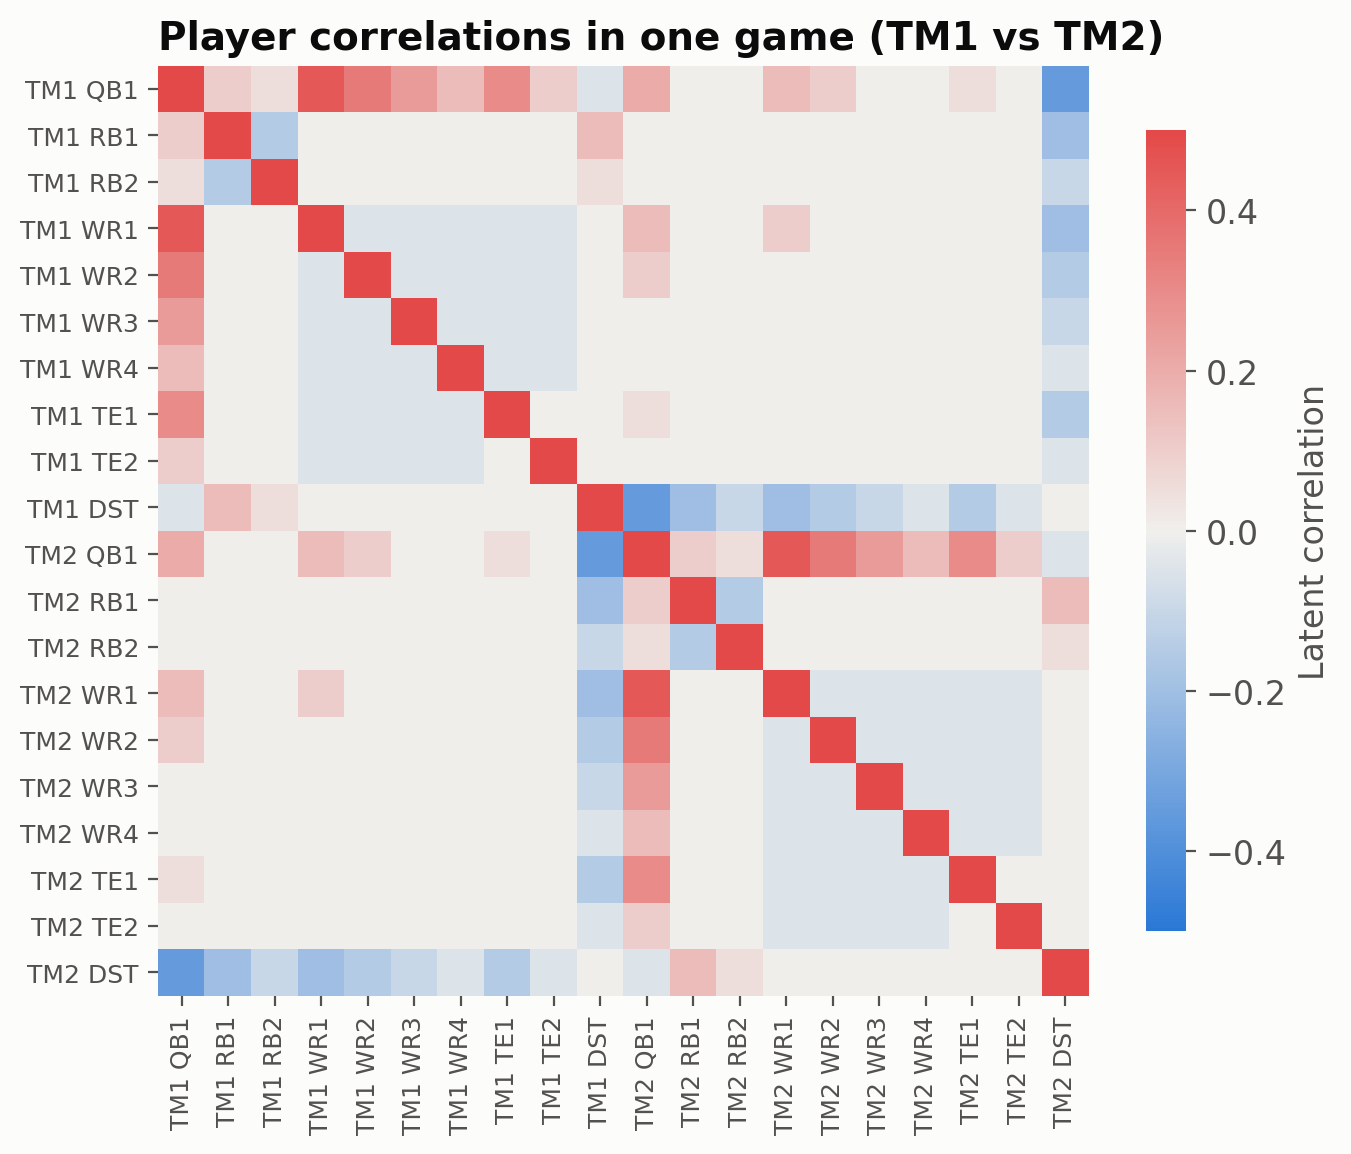
\includegraphics[width=\textwidth]{correlation_heatmap}
    \end{column}
    \begin{column}{0.62\textwidth}
      \begin{itemize}
        \setlength\itemsep{0.3em}
        \item 8 teams, 4 games, 80 fictional players with DraftKings-style salaries
        \item Correlations by position pair (QB--own WR1 $+0.45$, defense--opposing QB
          $-0.35$), repaired to be positive definite
        \item Gaussian copula with lognormal marginals, matched to each player's mean and SD:
          \quad $Z \sim N(0, R),\ \ X_i = e^{\,m_i + s_i Z_i}$
      \end{itemize}
      \vspace{0.2em}
      \centering
      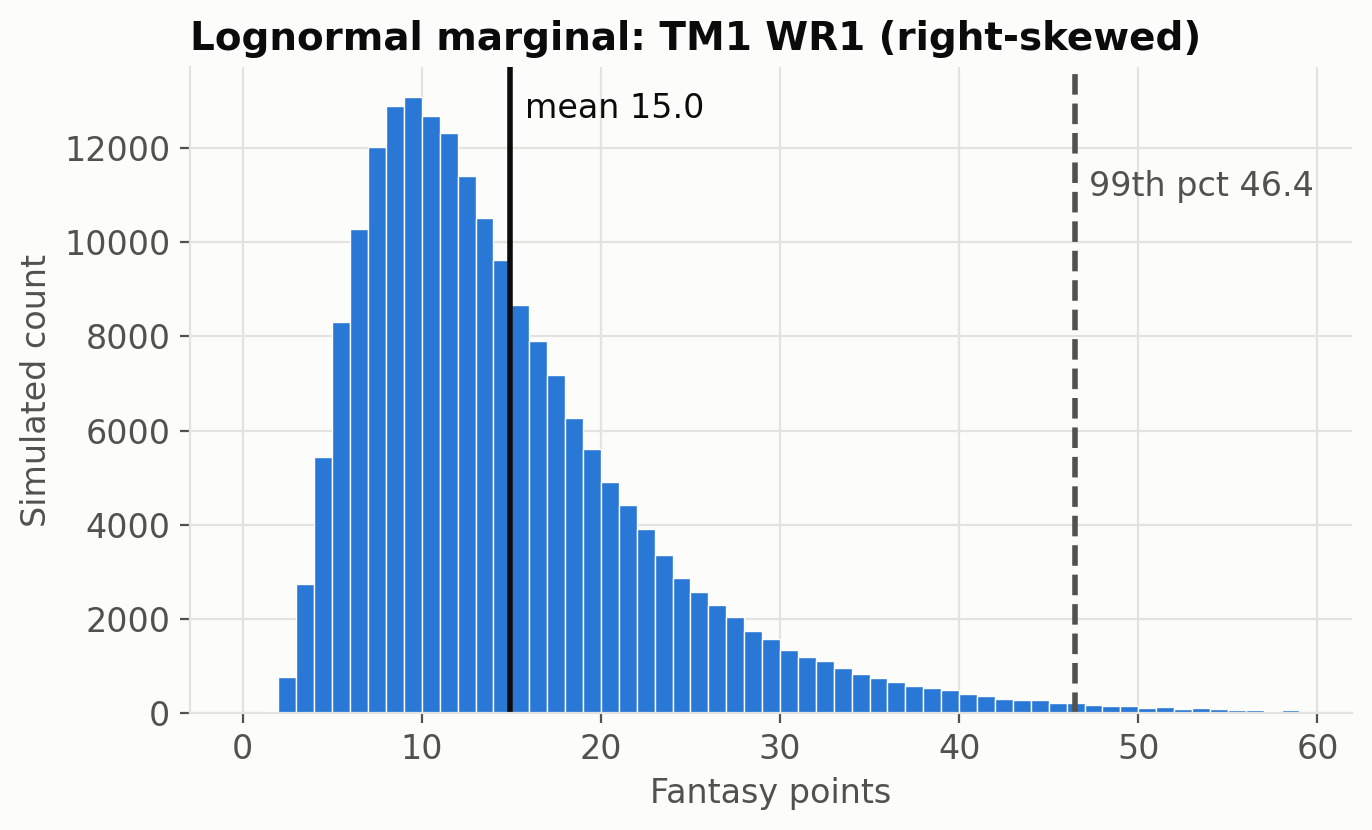
\includegraphics[width=0.62\textwidth]{marginal_wr1}
    \end{column}
  \end{columns}
\end{frame}

% ~1.5 min
\begin{frame}{Stage 2: a simulated field with realistic ``chalk''}
  \begin{columns}[c]
    \begin{column}{0.52\textwidth}
      \centering
      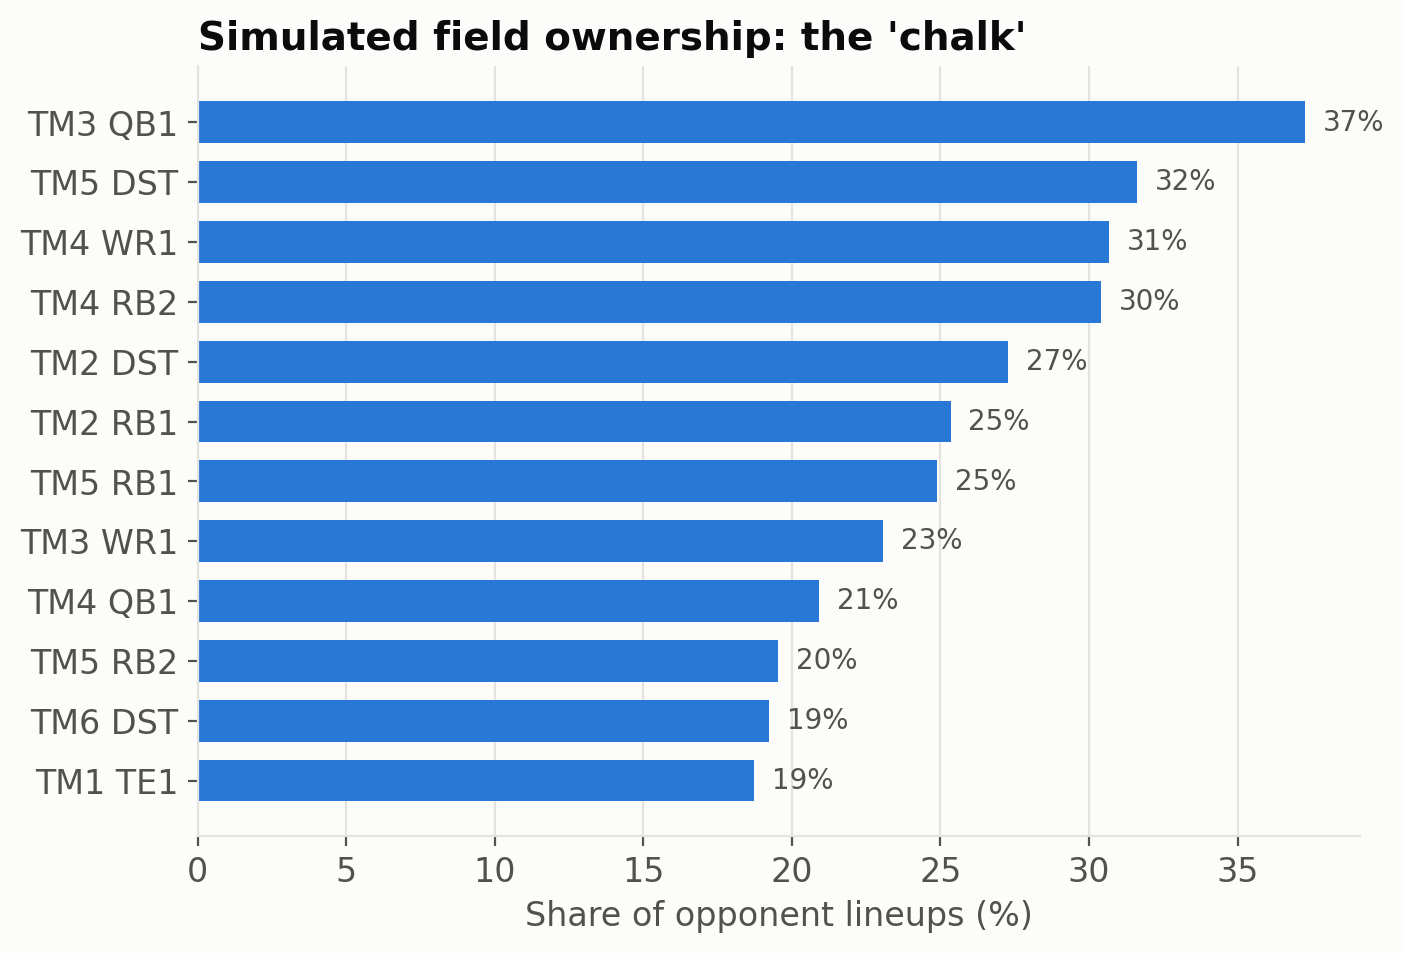
\includegraphics[width=\textwidth]{ownership}
    \end{column}
    \begin{column}{0.46\textwidth}
      \textbf{Minnows (80\,\%):} the paper's Algorithm 1
      \begin{itemize}
        \item $p_{\text{pos}} \sim \text{Dir}(\kappa\, p^0_{\text{pos}})$ per contest,
          $p^0 \propto \exp(\beta_1 z_{\text{proj}} + \beta_2 z_{\text{salary}})$
        \item Stack with probability $q = 0.35$
        \item Accept only if legal and salary $\ge$ \$49{,}000
      \end{itemize}
      \textbf{Sharks (20\,\%):} optimizer lineups on noisy projections
      \vspace{0.6em}

      \begin{tabular}{@{}ll@{}}
        Acceptance rate & 10\,\% \\
        Minnow stack rate & 32\,\% \\
        Avg.\ field projection & 91 (best: 103)
      \end{tabular}
    \end{column}
  \end{columns}
\end{frame}

% ~1.5 min
\begin{frame}{The objective: Upside CVaR, two ways}
  \vspace{-0.4em}
  \[
    \ucvar_\alpha(X) = \E\big[X \mid X \ge q_\alpha(X)\big]
    \approx \frac{1}{k}\sum_{s \in \text{top } k} X_s
  \]
  \vspace{-0.6em}
  \begin{center}\small the average of the best $(1-\alpha)$ share of simulated weeks\end{center}
  \begin{columns}[c]
    \begin{column}{0.42\textwidth}
      \begin{itemize}
        \setlength\itemsep{0.5em}
        \item \hl{S1, points only:} $X_s = w^\top \delta_s$
        \item \hl{S2, field-aware:} $X_s = w^\top \delta_s - G_{(0.1\%),s}$, our score minus
          the top-0.1\,\% score in the \emph{same} contest
        \item Candidates: lineup MILP $\max_w c^\top w$, with $c = \delta_s$ or
          $\mu + \lambda\sigma$
      \end{itemize}
    \end{column}
    \begin{column}{0.54\textwidth}
      \centering
      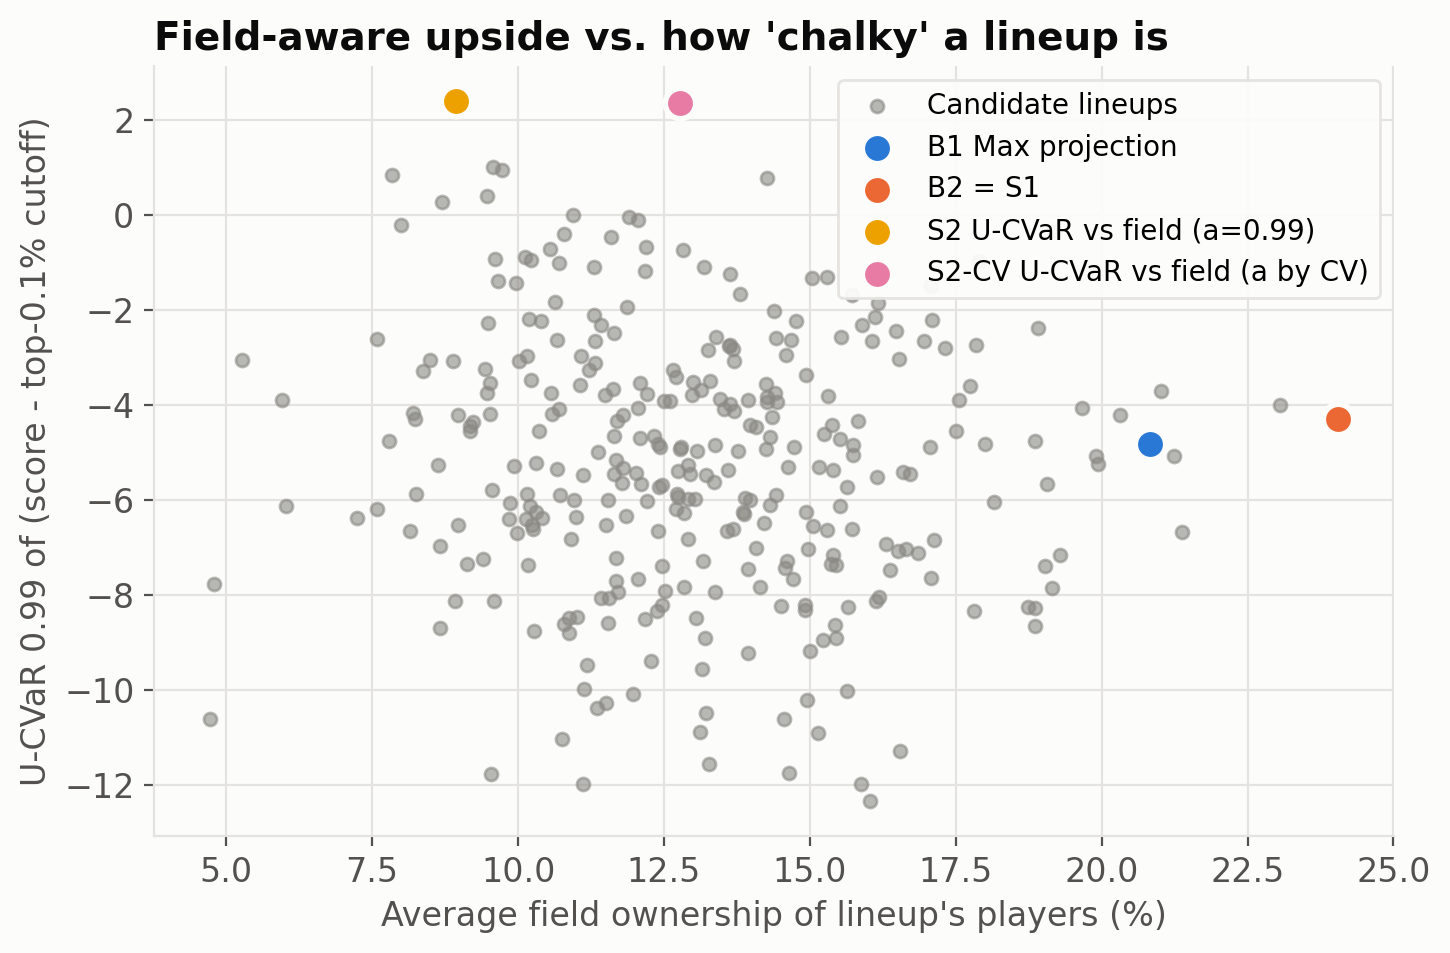
\includegraphics[width=0.92\textwidth]{pool_vs_ownership}
    \end{column}
  \end{columns}
\end{frame}

% ======================================================================
\section{Early results}

% ~1 min
\begin{frame}{Result 1: the contest simulator matches theory}
  A lineup drawn from the field is interchangeable with every opponent, so its expected
  return must be exactly the rake: $\E[\text{payout}] = (1 - 0.15) \times \$1$.
  \vspace{0.6em}
  \begin{columns}[c]
    \begin{column}{0.36\textwidth}
      \bigstat{$-15.9\,\%$}{simulated ROI, 95\,\% CI $-19.0\,\%$ to $-12.8\,\%$
      (theory $-15\,\%$), 400{,}000 held-out entries}
      \vspace{1.2em}

      \bigstat{19.9\,\%}{cash rate (theory 20\,\%); top-0.1\,\% rate 0.10\,\% (theory
      0.10\,\%)}
    \end{column}
    \begin{column}{0.62\textwidth}
      \centering
      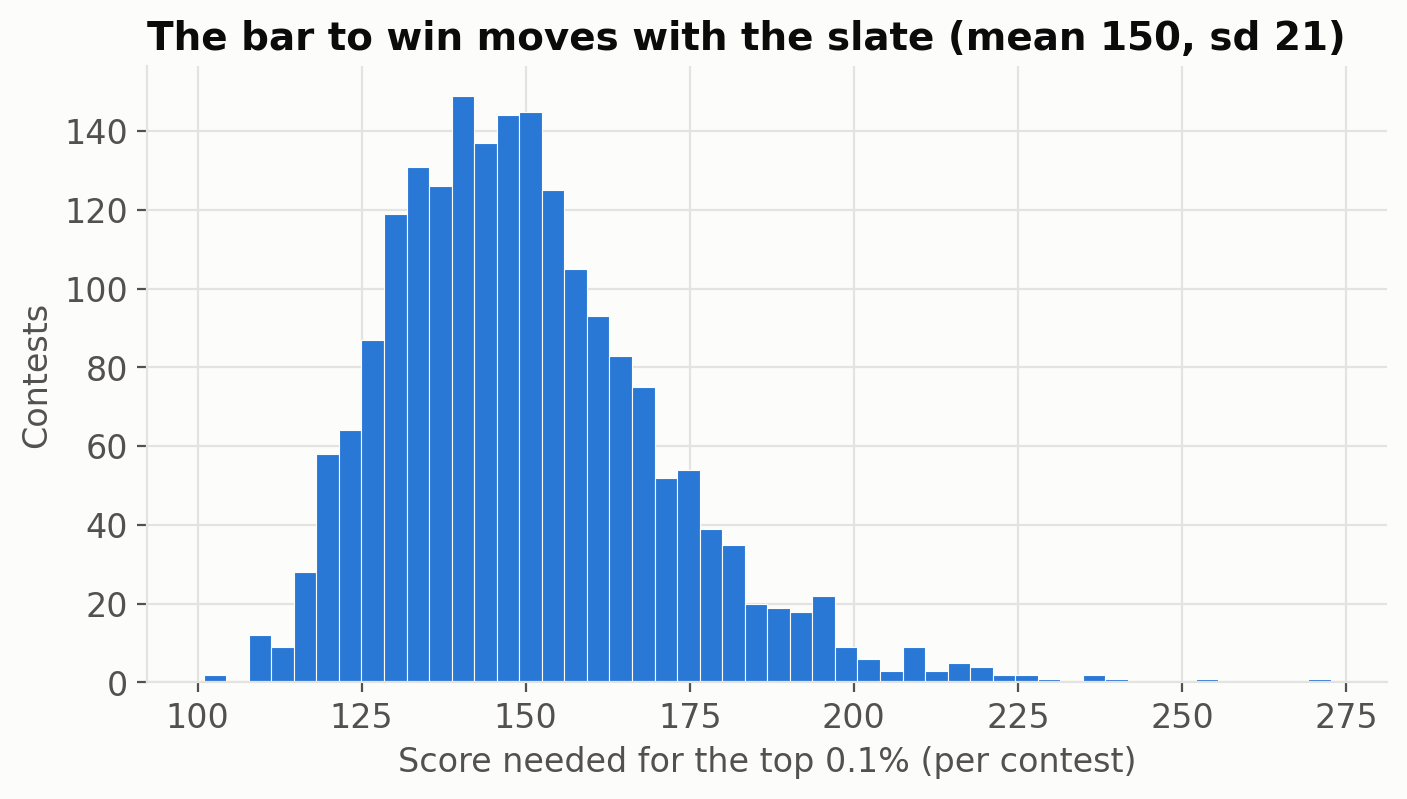
\includegraphics[width=\textwidth]{cutoff_distribution}
      {\footnotesize The winning line moves from contest to contest (mean 150, SD 21), so it
      must be simulated, not fixed.\par}
    \end{column}
  \end{columns}
  \vfill
  {\scriptsize\color{navy} All CIs are clustered by simulated field (200 fields $\times$ 10
  outcome draws).\par}
\end{frame}

% ~1.5 min
\begin{frame}{Result 2: field-aware upside wins the top spots}
  \centering
  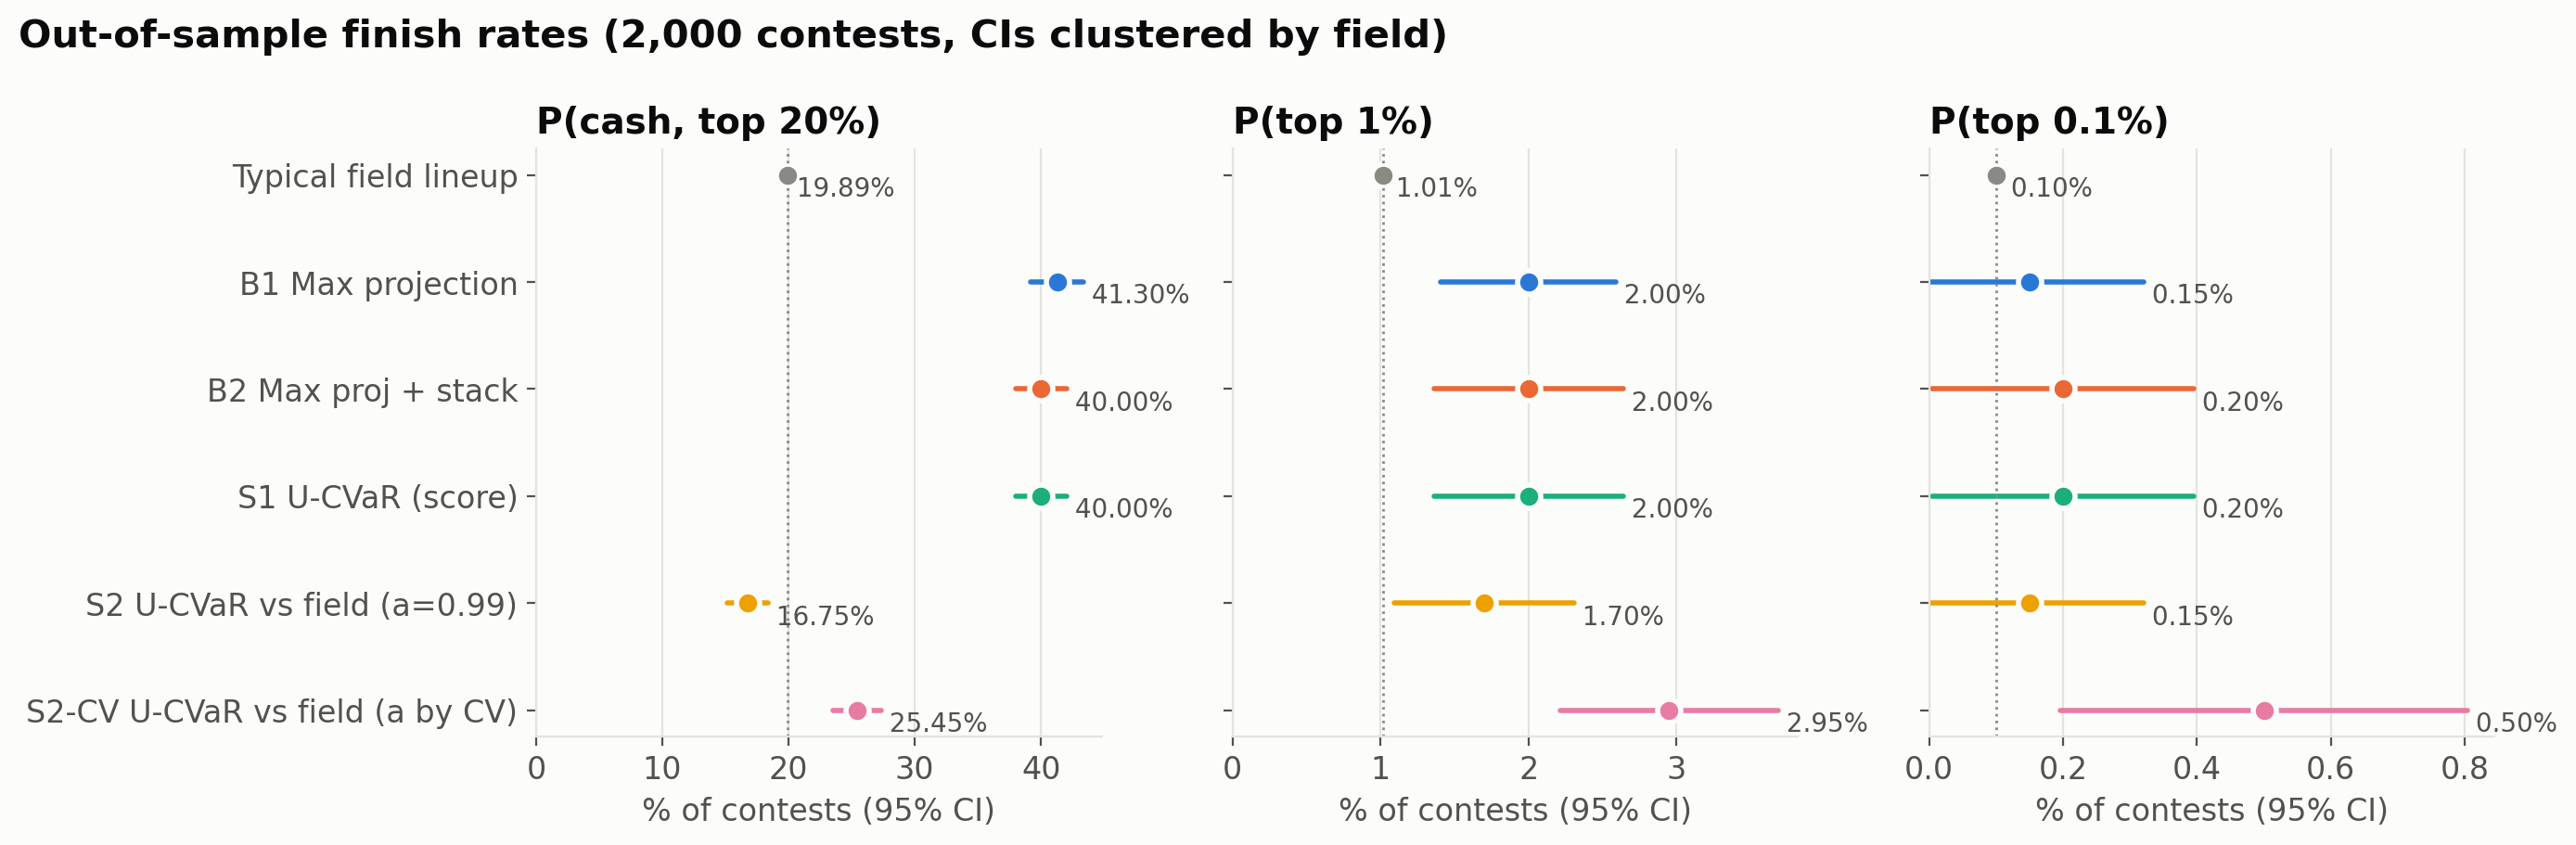
\includegraphics[width=0.92\textwidth]{results_finish_rates}
  \begin{itemize}
    \small
    \item \hl{Points-only (S1)} picked the same QB--WR stack as benchmark B2: no edge
    \item \hl{Field-aware, $\alpha$ by validation (S2-CV)} vs.\ max projection (paired):
      top 1\,\% $+0.95$ pts ($p = 0.04$), top 0.1\,\% $+0.35$ pts ($p = 0.052$), cashes
      16 pts less often; top-0.1\,\% rate 5$\times$ the field's ($p = 0.01$)
    \item The lineup is a \emph{game stack}: one team's QB, RB, WR1 plus the opponent's WR1
  \end{itemize}
\end{frame}

% ~1.5 min
\begin{frame}{Result 3: choosing on the far tail over-fits}
  \begin{columns}[c]
    \begin{column}{0.52\textwidth}
      \centering
      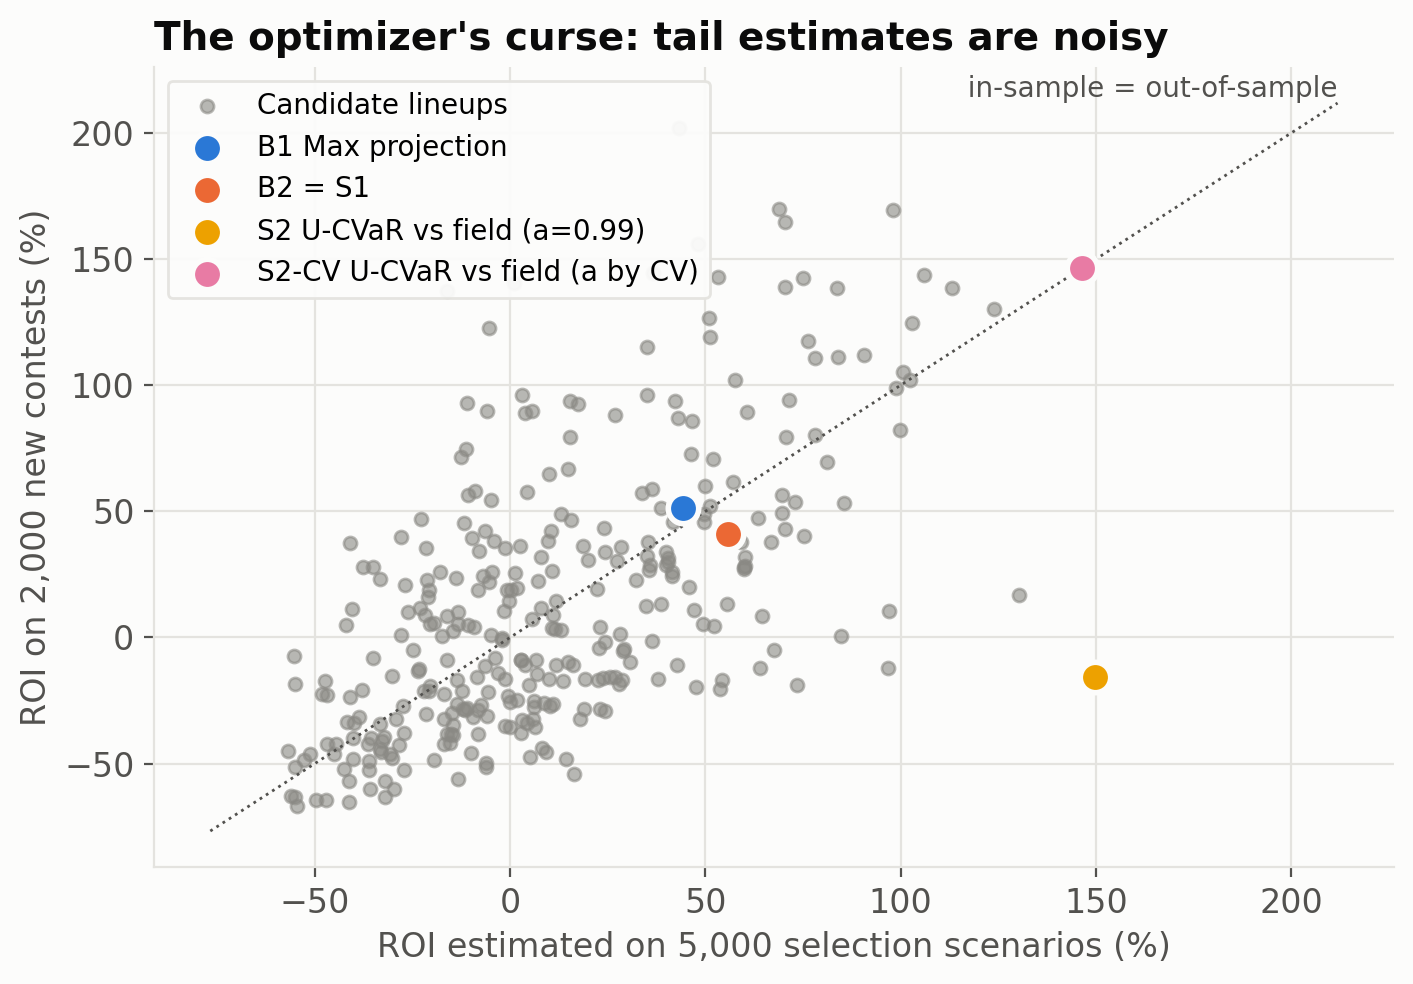
\includegraphics[width=\textwidth]{optimizers_curse}
    \end{column}
    \begin{column}{0.46\textwidth}
      \centering\small
      \begin{tabular}{@{}lrr@{}}
        \toprule
        Lineup & Est.\ ROI & Test ROI \\
        \midrule
        Max projection & $+44\,\%$ & $+51\,\%$ \\
        S2, $\alpha = 0.99$ & $+150\,\%$ & \textcolor{warn}{$-16\,\%$} \\
        S2-CV, $\alpha = 0.975$ & $+146\,\%$ & \textcolor{good}{$+146\,\%$} \\
        \bottomrule
      \end{tabular}
      \vspace{0.8em}
      \begin{itemize}
        \setlength\itemsep{0.3em}
        \item The 0.99 tail is only 50 scenarios
        \item \hl{Fix:} pick $\alpha$ on half the selection fields, check on the other half;
          test set never touched
        \item Field-aware U-CVaR still predicts test ROI best (corr.\ 0.62; projection 0.27)
        \item Payout gap vs.\ max projection: $+95$ pts, CI $[-17, +236]$, $p = 0.15$:
          \hl{not significant yet}
      \end{itemize}
    \end{column}
  \end{columns}
\end{frame}

% ~1 min
\begin{frame}{Result 4: importance sampling makes the tail cheaper}
  \begin{columns}[c]
    \begin{column}{0.47\textwidth}
      Estimate $p = P(\text{lineup score} > c)$. Draw $Z \sim N(\theta, R)$ and weight
      each draw by
      \[
        L(Z) = \frac{\varphi(Z;\,0,R)}{\varphi(Z;\,\theta,R)}
             = e^{-\theta^\top R^{-1} Z + \frac12 \theta^\top R^{-1}\theta}
      \]
      with $\theta = t\,Ra/\sqrt{a^\top R a}$ pointing toward our lineup's players.
      \vspace{0.6em}
      \begin{itemize}
        \setlength\itemsep{0.4em}
        \item \hl{8$\times$ fewer samples} for the same accuracy: IS with 250 draws matches
          crude MC with 2{,}000
        \item Gain grows as the event gets rarer: \hl{6$\times$ to 21$\times$}
      \end{itemize}
    \end{column}
    \begin{column}{0.51\textwidth}
      \centering
      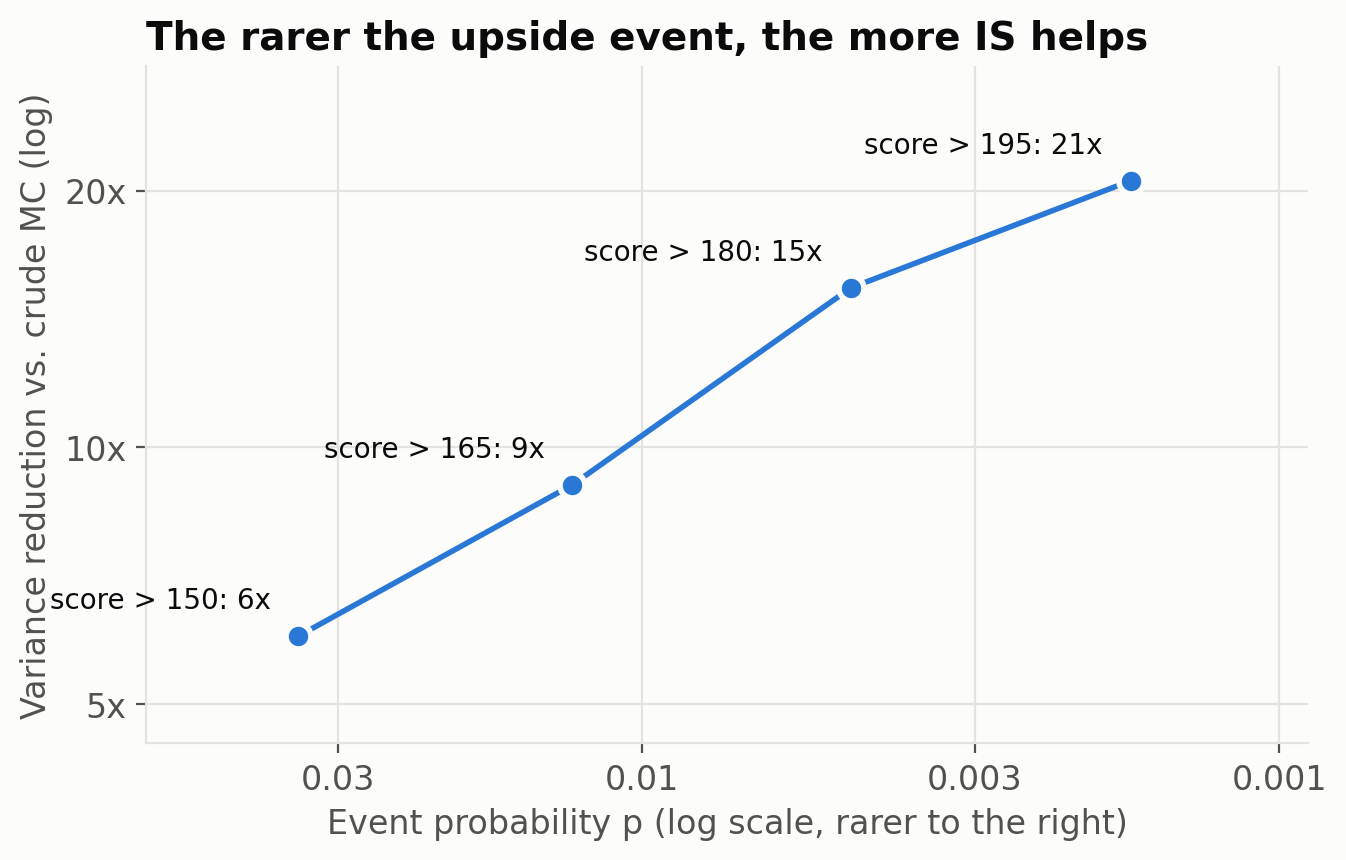
\includegraphics[width=\textwidth]{is_thresholds}
    \end{column}
  \end{columns}
\end{frame}

% ======================================================================
\section{What is next}

% ~0.5 min
\begin{frame}{What these early results do not show yet}
  \begin{columns}[t]
    \begin{column}{0.23\textwidth}
      \begin{block}{Synthetic slate}
        Realistic but made-up projections, salaries and correlations. One slate.
      \end{block}
    \end{column}
    \begin{column}{0.23\textwidth}
      \begin{block}{Smaller field}
        10{,}000 opponents instead of 100k+. The real top 0.1\,\% is 10$\times$ more
        crowded.
      \end{block}
    \end{column}
    \begin{column}{0.23\textwidth}
      \begin{block}{Single entry}
        Pros enter up to 150 lineups; the paper's biggest gains came from diversifying.
      \end{block}
    \end{column}
    \begin{column}{0.23\textwidth}
      \begin{block}{Noisy tail}
        Payout CIs are wide; two 1st places are a third of S2-CV's winnings.
      \end{block}
    \end{column}
  \end{columns}
\end{frame}

% ~1 min
\begin{frame}{Plan to the final report (due Dec 9)}
  \centering
  \begin{tabular}{@{}llp{0.52\textwidth}l@{}}
    \toprule
    & When & What & Who \\
    \midrule
    1 & Nov 25--30 & Real DraftKings slate; fitted distributions and correlations & Alex \\
    2 & Nov 27--Dec 2 & Dirichlet regression for ownership; calibrate field strength & Alex, Benjamin \\
    3 & Nov 28--Dec 3 & Multi-entry portfolios vs.\ the paper's mean--variance method & Benjamin \\
    4 & Nov 30--Dec 4 & Importance sampling \emph{inside} U-CVaR selection; more test contests & Alex, Marcus \\
    5 & Dec 2--5 & Sensitivity: $\alpha$, stacking rate, field size, payout curve & Marcus \\
    6 & Dec 3--9 & Final report, emailed by Dec 9, 5\,PM & Marcus, all \\
    \bottomrule
  \end{tabular}
  \vspace{1em}

  \textbf{Goal:} show whether the field-aware edge in expected payout becomes statistically
  significant.
\end{frame}

% ~1 min
\begin{frame}{Summary}
  \begin{itemize}
    \setlength\itemsep{0.9em}
    \item A working three-stage simulation of a 10{,}000-entry top-heavy contest that
      \hl{reproduces the $-15\,\%$ rake} for a typical entry
    \item Upside on \emph{points alone} recovers the obvious stacked lineup: no edge
    \item Upside measured \hl{against the simulated field} finds a low-owned game stack that
      reaches the top 1\,\% and top 0.1\,\% more often than max projection
    \item The far tail over-fits; validating $\alpha$ fixes it, and \hl{importance
      sampling} (up to 21$\times$) is how we will estimate it properly
  \end{itemize}
\end{frame}

\begin{frame}[plain]
  \centering\vfill
  {\Huge\bfseries\color{navy} Questions?}\par\vspace{1.5em}
  \small Every number in this talk: \texttt{python run\_all.py} (about 2 minutes)
  \vfill
\end{frame}

\end{document}
